% Z -> mumu cross section: review deck. House style of prompts/presentation_style.md rendered in beamer:
% 16:9, near-black #222222 page (= figure background), light-blue uppercase titles with a grey rule and page number,
% green secondary accent, drawn tables with a green best-value cell, cover with the headline result, numbered dividers.
\documentclass[aspectratio=169,9pt,t]{beamer}
\usepackage[T1]{fontenc}\usepackage[utf8]{inputenc}
\usepackage{helvet}\renewcommand{\familydefault}{\sfdefault}
\usepackage{amsmath,amssymb,graphicx,xcolor,colortbl,booktabs,tikz,textcase,array,multicol}
\usetikzlibrary{arrows.meta,positioning,shapes.misc}
\graphicspath{{figures/}}

% ---------------------------------------------------------------- palette (exact house values)
\definecolor{bg}{HTML}{222222}\definecolor{primary}{HTML}{2BA4DD}\definecolor{secondary}{HTML}{8AC63F}
\definecolor{rule}{HTML}{8C8C94}\definecolor{body}{HTML}{E6E6E6}\definecolor{muted}{HTML}{99999E}
\definecolor{best}{HTML}{577D29}\definecolor{rowA}{HTML}{252528}\definecolor{rowB}{HTML}{2F2F33}
\definecolor{cellb}{HTML}{666673}\definecolor{missing}{HTML}{CC4C4C}\definecolor{warn}{HTML}{E0A040}

\setbeamercolor{background canvas}{bg=bg}
\setbeamercolor{normal text}{fg=body,bg=bg}\setbeamercolor{structure}{fg=primary}
\setbeamercolor{itemize item}{fg=secondary}\setbeamercolor{itemize subitem}{fg=muted}
\setbeamercolor{enumerate item}{fg=secondary}
\setbeamertemplate{navigation symbols}{}
\setbeamertemplate{itemize item}{\raisebox{0.15ex}{\tiny$\blacksquare$}}
\setbeamertemplate{itemize subitem}{--}
\setbeamerfont{frametitle}{size=\large,series=\bfseries}
\setbeamersize{text margin left=0.7cm,text margin right=0.7cm}\setlength{\tabcolsep}{4pt}
\usefonttheme{professionalfonts}

% frame title: uppercase (math untouched), primary colour, thin rule, page number top right
\newcommand{\titlecolour}{primary}
\setbeamertemplate{frametitle}{%
  \vspace{0.3cm}%
  \begin{minipage}[t]{0.88\textwidth}\raggedright\color{\titlecolour}\bfseries\large\MakeTextUppercase{\insertframetitle}\end{minipage}%
  \hfill\begin{minipage}[t]{0.08\textwidth}\raggedleft\color{muted}\footnotesize\insertframenumber\end{minipage}\par
  \vspace{0.12cm}{\color{rule}\rule{\textwidth}{0.4pt}}\vspace{0.1cm}}
\setbeamertemplate{footline}{}

% section divider
\newcounter{divider}
\newcommand{\divider}[1]{\stepcounter{divider}\begin{frame}[plain]\vfill\centering
  {\color{primary}\bfseries\Large\MakeTextUppercase{\thedivider.\quad #1}}\\[0.35cm]{\color{rule}\rule{0.3\textwidth}{0.5pt}}\vfill\end{frame}}
% green-titled cross-check family
\newcommand{\greentitles}{\renewcommand{\titlecolour}{secondary}}\newcommand{\bluetitles}{\renewcommand{\titlecolour}{primary}}
% captions
\newcommand{\fcap}[1]{\par\vspace{0.05cm}{\color{secondary}\scriptsize #1\par}}
% tables
\newcolumntype{L}[1]{>{\raggedright\arraybackslash}p{#1}}
\newcolumntype{R}[1]{>{\raggedleft\arraybackslash}p{#1}}
\newcommand{\thead}{\rowcolor{primary}\color{bg}\bfseries}
\newcommand{\bestcell}[1]{\cellcolor{best}\textbf{#1}}
\newcommand{\warncell}[1]{\cellcolor{missing}\textbf{#1}}
\setlength{\arrayrulewidth}{0.3pt}\arrayrulecolor{cellb}
\renewcommand{\arraystretch}{1.25}
\newcommand{\tsize}{\scriptsize}
\newcommand{\pb}{\,\mathrm{pb}}
\newcommand{\muZ}{\mu_{Z}}
\newcommand{\met}{p_{T}^{\mathrm{miss}}}
\newcommand{\sfid}{\sigma_{\mathrm{fid}}}



\begin{document}

% ================================================================= cover
\begin{frame}[plain]
  \vspace{0.3cm}
  {\color{muted}\footnotesize\MakeTextUppercase{Niels ter Linden \;--\; BND school 2026 \;--\; Z$\to\mu\mu$ channel}}\\[0.15cm]
  {\color{rule}\rule{\textwidth}{0.5pt}}\\[0.35cm]
  {\color{primary}\bfseries\LARGE\MakeTextUppercase{The Z$\,\to\,\mu\mu$ cross section with CMS 2016 Open Data}}\\[0.25cm]
  {\color{body}\normalsize SingleMuon, Run2016G+H, 16.39 fb$^{-1}$ at 13 TeV \;--\; methods, results and validation \;--\; 15 September 2026}\\[0.3cm]
  \begin{minipage}[t]{0.6\textwidth}\footnotesize
    \textbf{Result} (dressed muons, $p_T > 26/20$ GeV, $|\eta| < 2.4$, $60 < m_{\mu\mu} < 120$ GeV):\\[0.1cm]
    {\color{secondary}\large $\sfid(pp\to Z/\gamma^*\to\mu\mu) = 790.1 \pm 0.2\,(\mathrm{stat}) \pm 8.5\,(\mathrm{syst}) \pm 9.6\,(\mathrm{lumi})\pb$}\\[0.15cm]
    $\muZ = 0.988 \pm 0.016$ relative to aMC@NLO (799.6 pb); $\sigma(60<m<120) = 1931 \pm 33\pb$; $\sigma(m>50) = 2002 \pm 34\pb$.\\[0.25cm]
    \textbf{How}
    \begin{itemize}\setlength\itemsep{0.1em}
      \item own skims of the NanoAOD parents; simulation for signal and prompt backgrounds, no QCD MC
      \item corrections measured in place: pileup, L1 prefiring, ID / isolation / trigger scale factors from tag-and-probe fits, muon momentum from the Z peak, non-prompt muons from a data-driven fake factor
      \item TRExFitter v1.8.0 profile-likelihood fit of $m_{\mu\mu}$ (12 $\times$ 5 GeV bins, 24 nuisance parameters), cross-checked by counting and by refits with other binnings
    \end{itemize}
  \end{minipage}\hfill
  \begin{minipage}[t]{0.34\textwidth}\footnotesize\color{muted}
    \textbf{\color{body}Sections}\\[0.1cm]
    1.\; Strategy and inputs\\
    2.\; Result and uncertainties\\
    3.\; Validation\\
    4.\; Conclusions\\[0.3cm]
    {\footnotesize Code and numbers: \texttt{z-mumu/} (\texttt{README.md}, \texttt{docs/09--15}, \texttt{output/v2/RESULTS\_v2.md}); review and fixes: \texttt{REVIEW.md}}
  \end{minipage}
\end{frame}

% ================================================================= 1. strategy
\divider{Strategy and inputs}

\begin{frame}{Strategy of the measurement}
  \centering
  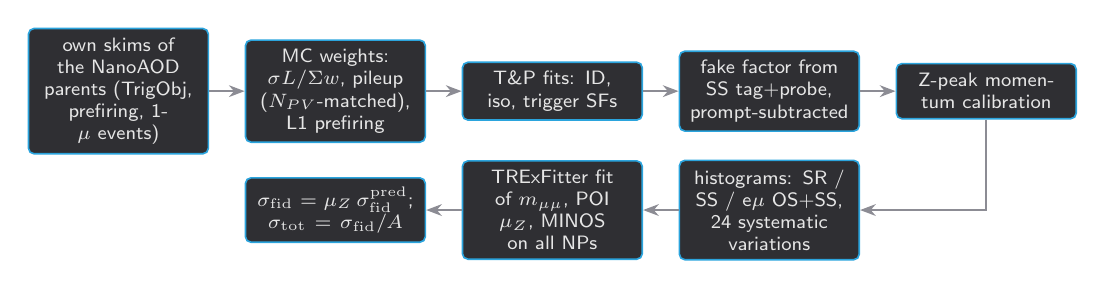
\begin{tikzpicture}[node distance=0.35cm and 0.45cm, every node/.style={font=\scriptsize},
      box/.style={draw=primary, rounded corners=2pt, text=body, fill=rowB, minimum height=0.7cm, text width=2.05cm, align=center, line width=0.6pt},
      arr/.style={-{Stealth[length=2mm]}, draw=rule, line width=0.6pt}]
    \node[box] (skim) {own skims of the NanoAOD parents (TrigObj, prefiring, 1-$\mu$ events)};
    \node[box, right=of skim] (w) {MC weights: $\sigma L/\Sigma w$, pileup ($N_{PV}$-matched), L1 prefiring};
    \node[box, right=of w] (tnp) {T\&P fits: ID, iso, trigger SFs};
    \node[box, right=of tnp] (ff) {fake factor from SS tag+probe, prompt-subtracted};
    \node[box, right=of ff] (mom) {Z-peak momentum calibration};
    \node[box, below=of ff] (hist) {histograms: SR / SS / e$\mu$ OS+SS, 24 systematic variations};
    \node[box, left=of hist] (trex) {TRExFitter fit of $m_{\mu\mu}$, POI $\muZ$, MINOS on all NPs};
    \node[box, left=of trex] (xs) {$\sfid = \muZ\,\sfid^{\mathrm{pred}}$; $\sigma_{\mathrm{tot}} = \sfid/A$};
    \draw[arr] (skim) -- (w); \draw[arr] (w) -- (tnp); \draw[arr] (tnp) -- (ff); \draw[arr] (ff) -- (mom);
    \draw[arr] (mom) |- (hist); \draw[arr] (hist) -- (trex); \draw[arr] (trex) -- (xs);
  \end{tikzpicture}
  \vspace{0.15cm}\footnotesize
  \begin{columns}[T]
    \begin{column}{0.5\textwidth}
      \textbf{Selection (signal region)}
      \begin{itemize}\scriptsize
        \item \texttt{HLT\_IsoMu24 || HLT\_IsoTkMu24}, MET filters, $N_{PV}\ge1$
        \item exactly two tight muons (\texttt{tightId}, iso $<0.15$, $|d_{xy}|<0.2$, $|d_z|<0.5$ cm), $p_T > 26/20$, $|\eta|<2.4$, $\geq 1$ trigger-matched, opposite sign
        \item FSR-recovered $60 < m_{\mu\mu} < 120$ GeV: 10\,378\,567 data events, 99.3\,\% signal
      \end{itemize}
    \end{column}
    \begin{column}{0.48\textwidth}
      \textbf{Fiducial volume and normalisation}
      \begin{itemize}\scriptsize
        \item dressed muons ($\Delta R<0.1$), $p_T > 26/20$, $|\eta|<2.4$, $60<m<120$ GeV; $C = 0.7914$, $A_{60\text{--}120} = 0.4092$ (aMC@NLO)
        \item $\sigma(Z/\gamma^*\to\ell\ell, m>50) = 6077.22/3$ pb, $L = 16393.381$ pb$^{-1}$ (normtag)
        \item backgrounds: Z$\to\tau\tau$, t$\bar{\mathrm{t}}$, tW, WW, WZ, ZZ from MC (0.62\,\%), non-prompt from data (0.04\,\%)
      \end{itemize}
    \end{column}
  \end{columns}
\end{frame}

\begin{frame}{Tag-and-probe: trigger and identification efficiencies}
  \centering
\includegraphics[height=0.36\textheight]{tnp_trigger.pdf}\\[0.05cm]
  
\includegraphics[height=0.36\textheight]{tnp_eff_id.pdf}
  \fcap{20.1 M tag-probe pairs. Trigger: trigger-object matching, per-muon plateau 0.907 (data) / 0.923 (MC), applied per event as $1-(1-\epsilon_1)(1-\epsilon_2)$. Tight ID: simultaneous pass/fail fits (DY template $\otimes$ Gaussian + exponential); the MC fit closes on the gen-matched truth to $-0.1$\,\%.}
\end{frame}

\begin{frame}{Tag-and-probe: scale-factor maps}
  \begin{columns}[T]
    \begin{column}{0.49\textwidth}\centering
\includegraphics[width=\textwidth]{tnp_sf_id_map.pdf}\fcap{tight ID: 0.97--0.99, $\langle\mathrm{SF}\rangle = 0.980$}\end{column}
    \begin{column}{0.49\textwidth}\centering
\includegraphics[width=\textwidth]{tnp_sf_iso_map.pdf}\fcap{isolation: 1.00--1.04, $\langle\mathrm{SF}\rangle = 1.006$, flat in pileup (half-spread 0.003)}\end{column}
  \end{columns}
  \small Systematic variants (background model, fit range, tag selection, powheg templates) enter as the \texttt{MuonID} / \texttt{MuonIso} / \texttt{MuonTrigger} nuisance parameters, coherent over all cells. Muon reconstruction (track $\to$ muon) is not measurable in NanoAOD: external $0.4\,\%$ per muon, correlated, i.e. 0.8\,\% per event.
\end{frame}

\begin{frame}{Non-prompt muons and momentum calibration}
  \centering
\includegraphics[height=0.42\textheight]{ff_map_and_closure.pdf}\\[0.05cm]
  
\includegraphics[height=0.28\textheight]{momentum_zpeak.pdf}
  \fcap{Fake factor $N_{\mathrm{tight}}/N_{\mathrm{anti\text{-}tight}}$ from same-sign tag+probe pairs with prompt MC subtracted: SR non-prompt 3\,870 $\pm$ 80 (stat) $\pm$ 30\,\% (method); same-sign closure 2094 $\pm$ 20 predicted vs 1932 $\pm$ 79 observed. Momentum: scale $\kappa$ and extra smearing per $|\eta|$ from Breit--Wigner $\otimes$ Gaussian fits of the Z peak (data vs MC); propagated as \texttt{MuonScale} / \texttt{MuonRes}.}
\end{frame}

\begin{frame}{Pileup: the profile is fitted to the vertex multiplicity}
  \begin{columns}[T]
    \begin{column}{0.48\textwidth}\centering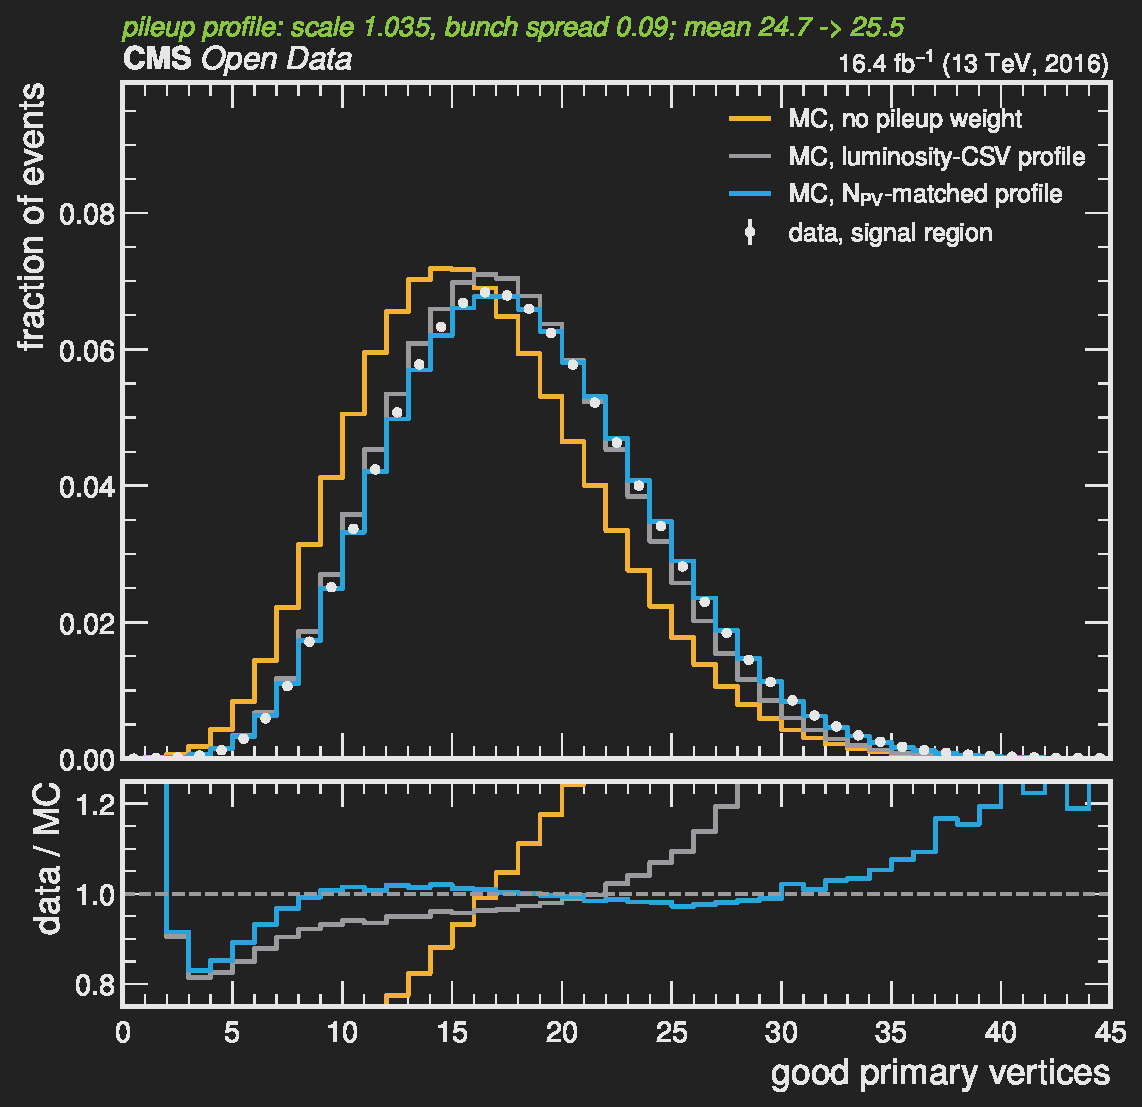
\includegraphics[height=0.72\textheight]{pileup_match.pdf}\end{column}
    \begin{column}{0.5\textwidth}\footnotesize\vspace{0.2cm}
      \begin{itemize}\setlength\itemsep{0.35em}
        \item No official \texttt{puWeights} file is reachable; the data profile comes from the per-lumisection \texttt{avgpu} of the Open Data luminosity record ($\times\,69.2/80$ mb).
        \item That raw profile has no bunch-to-bunch spread and is $\approx$ 4\,\% too low: data/MC in $N_{PV}$ rose from 0.8 to 1.2 (grey).
        \item Two parameters -- a scale of the per-lumisection mean and a relative Gaussian spread -- are fitted to the signal-region $N_{PV}$ distribution: scale 1.035, spread 9\,\%; $\chi^2/\mathrm{ndf}$ 104\,414 $\to$ 4\,729 / 50 (blue).
        \item The \texttt{Pileup} nuisance parameter ($\sigma_{\mathrm{mb}} \pm 4.6\,\%$) is then pulled by $+0.06\sigma$ instead of $-1.5\sigma$; impact on $\sfid$ 0.13\,\%.
      \end{itemize}
    \end{column}
  \end{columns}
\end{frame}

\begin{frame}{Signal region: mass spectrum}
  \begin{columns}[T]
    \begin{column}{0.44\textwidth}\centering
\includegraphics[height=0.7\textheight]{sr_mass.pdf}\end{column}
    \begin{column}{0.44\textwidth}\centering
\includegraphics[height=0.7\textheight]{sr_mass_log.pdf}\end{column}
  \end{columns}
  \fcap{10\,378\,567 data events; prompt MC + fake factor 10\,442\,328 pre-fit ($\muZ = 1$). The 3\,\% deficit at 60--80 GeV is a lineshape difference between the data and aMC@NLO (section 2).}
\end{frame}

% ================================================================= 2. result
\divider{Result and uncertainties}

\begin{frame}{Cross section: fit, counting and references}
  \begin{columns}[T]
    \begin{column}{0.5\textwidth}\centering
      
\includegraphics[width=0.97\textwidth]{summary_sigma.pdf}
    \end{column}
    \begin{column}{0.48\textwidth}\tsize
      \begin{tabular}{L{3.8cm}R{2.4cm}}
        \thead quantity & value\\
        \rowcolor{rowA} $\sfid$ (fit, 12 $\times$ 5 GeV) & \bestcell{$790.1 \pm 12.6\pb$}\\
        \rowcolor{rowB} $\sfid$ (counting $(N-B)/(CL)$) & $794.7\pb$\\
        \rowcolor{rowA} $\muZ$ & $0.988\,^{+0.016}_{-0.016}$\\
        \rowcolor{rowB} goodness of fit (12 bins) & $p = 0.79$\\
        \rowcolor{rowA} $\sigma(60<m<120)$, $A=0.4092$ & $1931 \pm 33\pb$\\
        \rowcolor{rowB} $\sigma(m>50)$, $A=0.3947$ & $2002 \pm 34\pb$\\
        \rowcolor{rowA} $C$ (reco / fiducial) & 0.7914\\
        \rowcolor{rowB} aMC@NLO $\sfid^{\mathrm{pred}}$ & $799.6\pb$\\
        \rowcolor{rowA} external reviewer, same volume & $797.2\pb$\\
      \end{tabular}\\[0.3cm]
      \begin{itemize}\footnotesize
        \item $\sfid = \muZ \times \sfid^{\mathrm{pred}}$; algebraically $(N - B)/(L\,C)$, so the assumed DY cross section cancels.
        \item Fit and counting differ by 0.6\,\%: the shape information moves the lineshape and momentum nuisance parameters (next slides).
        \item The data statistical uncertainty is 0.03\,\%; the effective statistical limit is the MC (0.38\,\%).
      \end{itemize}
    \end{column}
  \end{columns}
\end{frame}

\begin{frame}{Uncertainty budget and stability}
  \begin{columns}[T]
    \begin{column}{0.42\textwidth}\tsize
      \begin{tabular}{L{3.1cm}R{1.1cm}L{0.8cm}}
        \thead group & on $\muZ$ & corr.\\
        \rowcolor{rowA} luminosity (external) & 1.20\,\% & yes\\
        \rowcolor{rowB} muon efficiency (reco 0.77\,\%) & 0.87\,\% & $\mu$ ch.\\
        \rowcolor{rowA} L1 prefiring & 0.51\,\% & yes\\
        \rowcolor{rowB} signal modelling & 0.49\,\% & yes\\
        \rowcolor{rowA} MC statistics & 0.38\,\% & no\\
        \rowcolor{rowB} muon momentum & 0.37\,\% & $\mu$ ch.\\
        \rowcolor{rowA} pileup & 0.13\,\% & yes\\
        \rowcolor{rowB} background normalisation & 0.08\,\% & yes\\
        \rowcolor{rowA} non-prompt & 0.04\,\% & no\\
        \rowcolor{rowB} data statistics & 0.03\,\% & no\\
        \rowcolor{rowA} \textbf{total} & \textbf{1.57\,\%} & \\
      \end{tabular}
      \fcap{1.06\,\% without the luminosity. Acceptance for $\sigma_{\mathrm{tot}}$: 0.61\,\% (PDF, scales, $\alpha_s$).}
    \end{column}
    \begin{column}{0.56\textwidth}\centering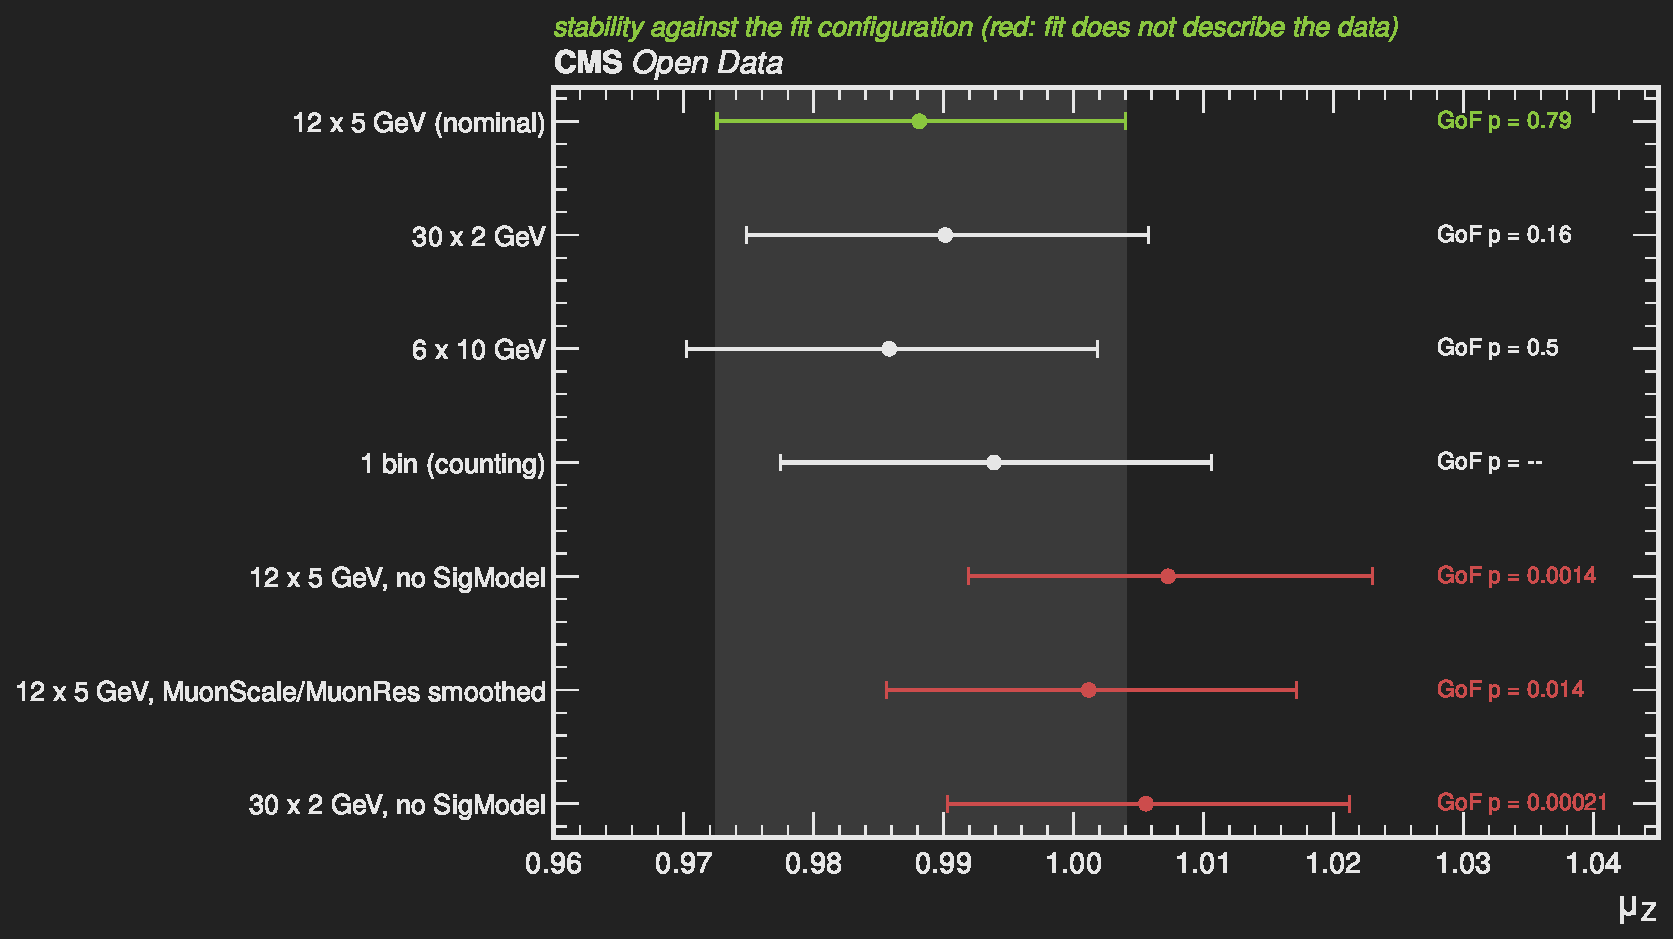
\includegraphics[width=\textwidth]{stability.pdf}
      \fcap{The binnings that describe the data agree within $\pm 0.2$\,\%. Dropping the generator template or smoothing the momentum templates gives fits with $p \le 0.01$: rejected.}
    \end{column}
  \end{columns}
\end{frame}

\begin{frame}{Nuisance parameters: pulls, constraints, ranking}
  \begin{columns}[T]
    \begin{column}{0.48\textwidth}\centering
\includegraphics[height=0.72\textheight]{fit_pulls.pdf}\end{column}
    \begin{column}{0.5\textwidth}\centering
\includegraphics[height=0.72\textheight]{fit_ranking.pdf}\end{column}
  \end{columns}
  \fcap{MINOS on every parameter. Only the three shape parameters are constrained by the 10 M-event spectrum: \texttt{SigModel} $+0.66$ (0.14), \texttt{MuonScale} $-0.48$ (0.14), \texttt{MuonRes} $+0.40$ (0.12); everything else within $\pm 0.8\sigma$ at its prior width. Luminosity and muon reconstruction dominate the ranking.}
\end{frame}

\begin{frame}{The signal lineshape: two generators, and the data in between}
  \begin{columns}[T]
    \begin{column}{0.5\textwidth}\centering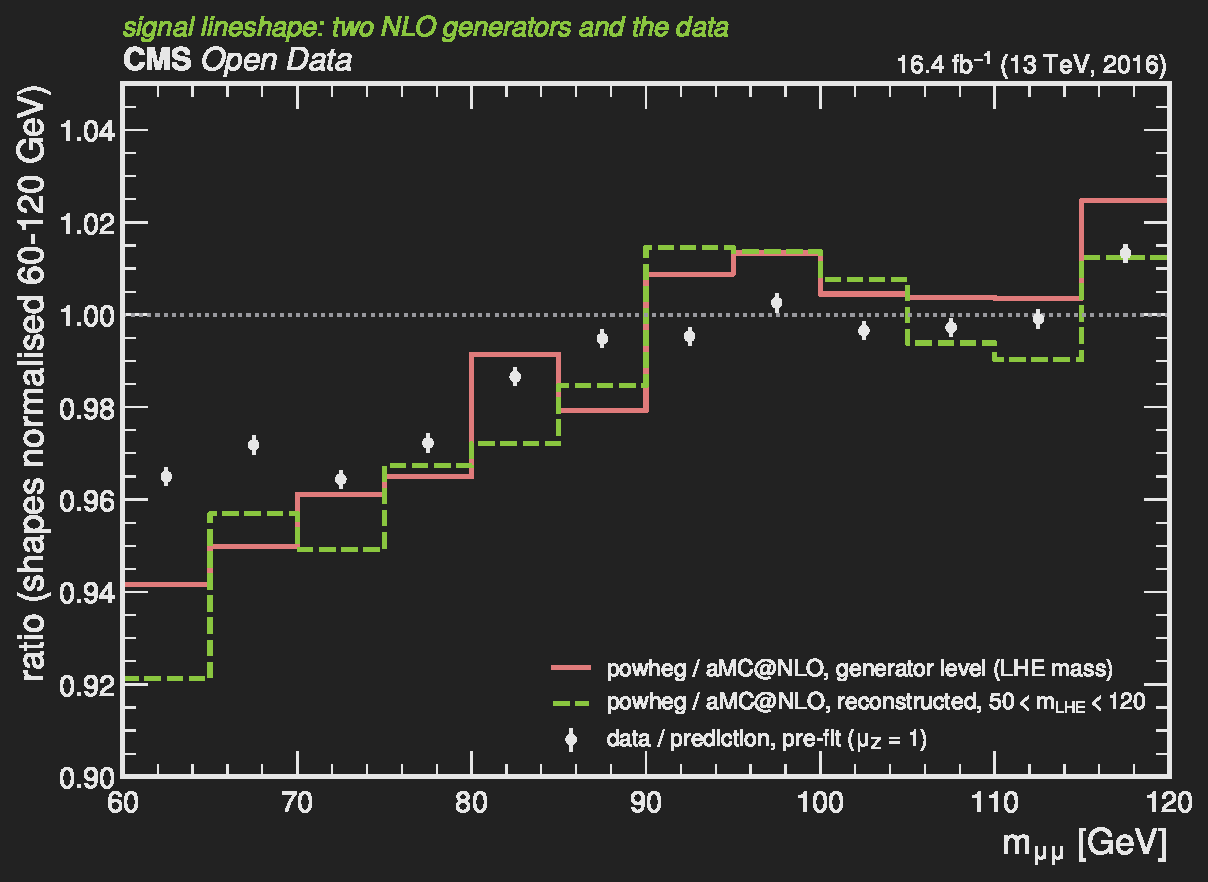
\includegraphics[width=\textwidth]{lineshape.pdf}\end{column}
    \begin{column}{0.5\textwidth}\centering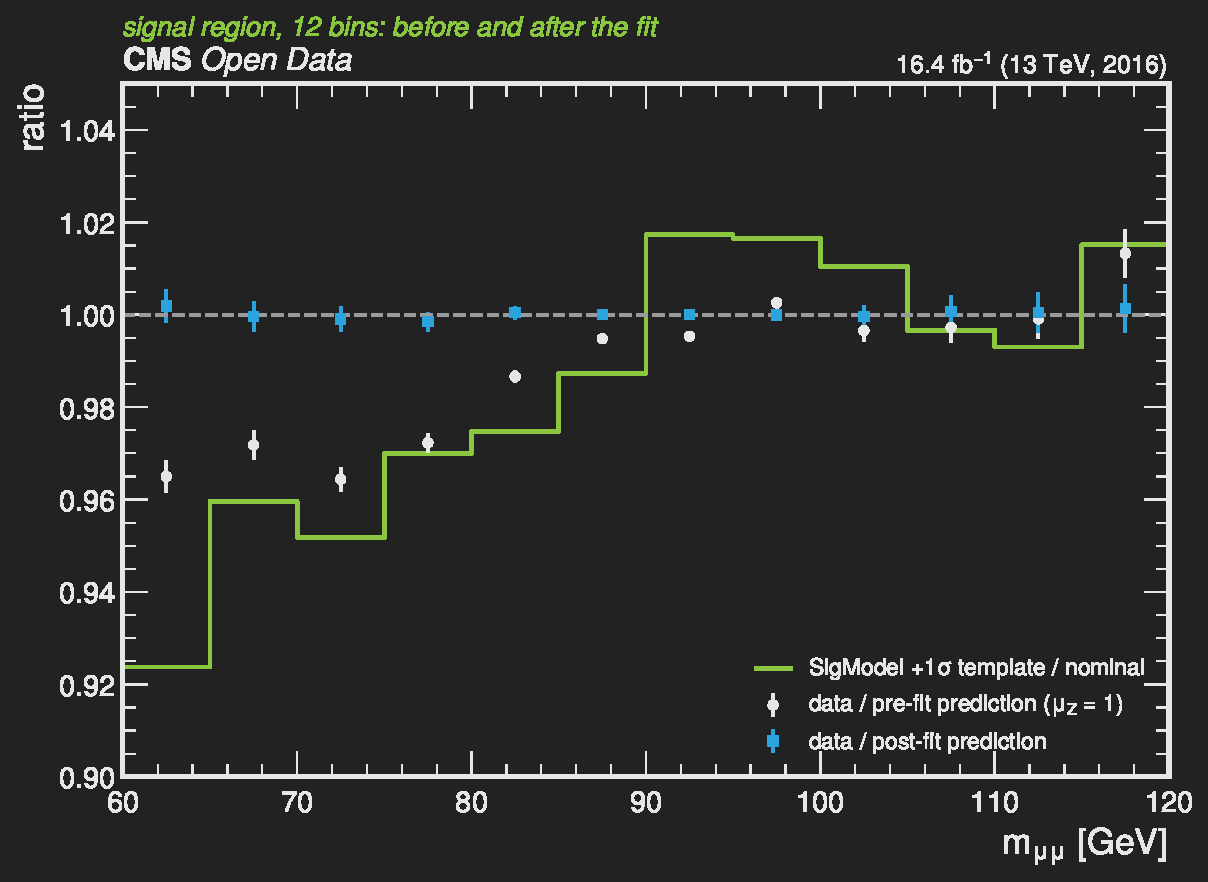
\includegraphics[width=\textwidth]{postfit_ratio.pdf}\end{column}
  \end{columns}
  \fcap{Left: powheg has 4--6\,\% less continuum than aMC@NLO below 80 GeV already at Born level; the data sit between the two. Right: the two-sided \texttt{SigModel} template (powheg / aMC@NLO inside the common $50 < m_{\mathrm{LHE}} < 120$ GeV window) lets the fit absorb it with a $+0.66\sigma$ pull; post-fit the spectrum is described within 0.3\,\% in every bin.}
\end{frame}

% ================================================================= 3. validation
\divider{Validation}

\begin{frame}{e$\mu$ regions: flavour-symmetric backgrounds and non-prompt electrons}
  \begin{columns}[T]
    \begin{column}{0.33\textwidth}\centering
\includegraphics[width=\textwidth]{cr_pt_el.pdf}\end{column}
    \begin{column}{0.33\textwidth}\centering
\includegraphics[width=\textwidth]{cr_njet.pdf}\end{column}
    \begin{column}{0.33\textwidth}\centering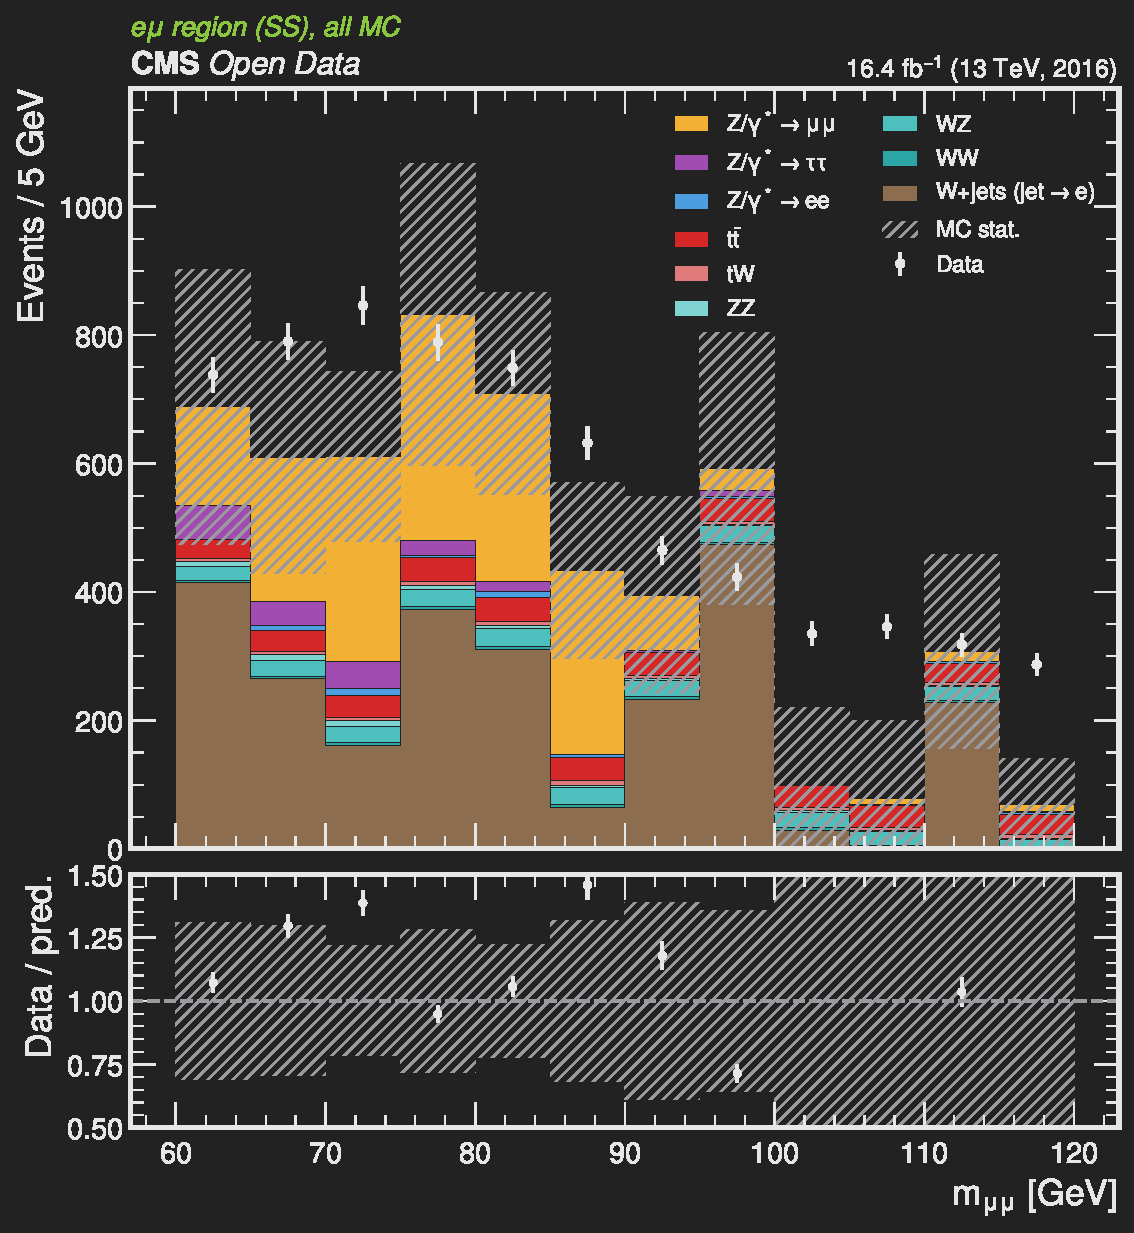
\includegraphics[width=\textwidth]{ssemu_mass.pdf}\end{column}
  \end{columns}
  \fcap{One tight matched muon + one medium electron, $60 < m_{e\mu} < 120$ GeV. Opposite sign: 72\,357 data vs 72\,959 predicted (0.992), t$\bar{\mathrm{t}}$ 43\,165, Z$\to\tau\tau$ 13\,914, WW 5\,274, tW 4\,113, non-prompt electrons (W+jets, Z$\to\mu\mu$+conversion) $\approx$ 6\,000. Same sign (right): 6\,718 vs 5\,428, the charge-symmetric non-prompt part, limited by W+jets MC statistics and the absent QCD sample. Validation only (not in the fit).}
\end{frame}

\begin{frame}{Signal-region distributions}
  \begin{columns}[T]
    \begin{column}{0.25\textwidth}\centering
\includegraphics[width=\textwidth]{sr_npv.pdf}\end{column}
    \begin{column}{0.25\textwidth}\centering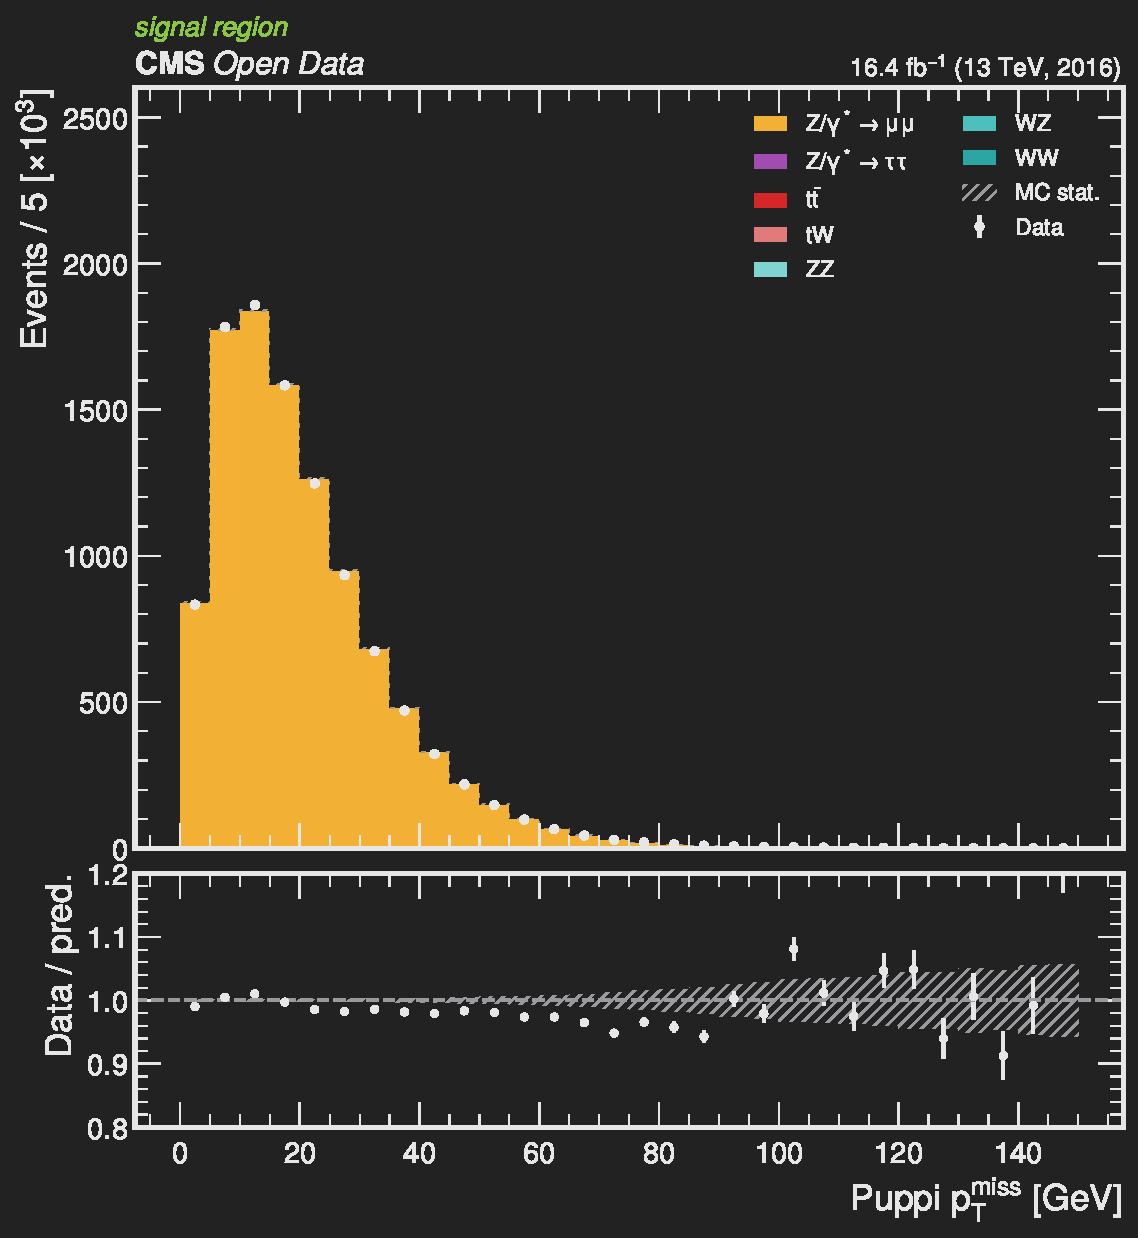
\includegraphics[width=\textwidth]{sr_puppimet.pdf}\end{column}
    \begin{column}{0.25\textwidth}\centering
\includegraphics[width=\textwidth]{sr_njet.pdf}\end{column}
    \begin{column}{0.25\textwidth}\centering
\includegraphics[width=\textwidth]{sr_zpt.pdf}\end{column}
  \end{columns}
  \fcap{Pileup after the matched profile; Puppi $\met$ (PF $\met$ is broader in data: MC jets are not JER-smeared and the unclustered energy is mismodelled -- neither is used); lepton-cleaned jets; $p_T^{\mu\mu}$ shows the known aMC@NLO+Pythia8 low-$p_T$ mismodelling, which enters $C$ through the $p_T$ thresholds and is covered by the generator comparison.}
\end{frame}

\begin{frame}{What the review changed (same day)}
  \footnotesize\vspace{0.2cm}
  \begin{tabular}{L{4.5cm}L{5.7cm}L{2.7cm}}
    \thead finding & fix & effect on the result\\
    \rowcolor{rowA} e$\mu$ region +9\,\%: non-prompt electrons removed by the prompt-only MC filter & keep all MC in the e$\mu$ regions, add W+jets and a same-sign e$\mu$ region & none (validation)\\
    \rowcolor{rowB} 30 $\times$ 2 GeV fit not robust ($\pm$0.8\,\% with binning / templates), over-constrained NPs, one-sided \texttt{SigModel} with a generator-cut artefact & 12 $\times$ 5 GeV, no smoothing, two-sided \texttt{SigModel} inside the common LHE window, MINOS on all parameters, stability table & 791.8 $\to$ 790.1 pb; stable to $\pm$0.2\,\%\\
    \rowcolor{rowA} pileup profile 4\,\% low, \texttt{Pileup} pulled $-1.5\sigma$ & profile fitted to $N_{PV}$ & pull $+0.06\sigma$\\
    \rowcolor{rowB} \texttt{MuonReco} 0.4\,\% per event instead of per muon & 0.8\,\% per event & syst 1.40 $\to$ 1.57\,\%\\
    \rowcolor{rowA} jets not lepton-cleaned; $\met$ broader in data & cleaned jets; Puppi $\met$ shown, nothing else needed & none\\
  \end{tabular}
  \fcap{Full account with reasoning: \texttt{z-mumu/REVIEW.md} (section 0 = status after the fixes).}
\end{frame}

% ================================================================= 4. conclusions
\divider{Conclusions}

\begin{frame}{Conclusions}
  \begin{columns}[T]
    \begin{column}{0.55\textwidth}\footnotesize
      \begin{itemize}\setlength\itemsep{0.4em}
        \item {\color{secondary}$\sfid(pp\to Z/\gamma^*\to\mu\mu) = 790.1 \pm 0.2 \pm 8.5 \pm 9.6\pb$}, 1.6\,\% total, in agreement with aMC@NLO (799.6 pb, $\muZ = 0.988 \pm 0.016$) and with an independent analysis of the same data (797.2 pb).
        \item Every correction is measured in the data itself (efficiencies, momentum scale, pileup, non-prompt background); the only external inputs are the luminosity (1.2\,\%) and the muon reconstruction efficiency (0.4\,\%/muon) -- together 1.4 of the 1.6\,\%.
        \item The profile-likelihood fit is validated three ways: goodness of fit $p = 0.79$, stability of $\muZ$ against the binning ($\pm 0.2$\,\%), and the counting cross-check (794.7 pb).
        \item The e$\mu$ regions validate the flavour-symmetric backgrounds to 1\,\%; the same-sign regions validate the non-prompt estimate.
        \item Inputs for the combination: \texttt{fit/fitinputs/zmumu.root}, \texttt{fit/zmumu.config} (POI \texttt{mu\_Z}, correlated NP names per \texttt{fitting/CONVENTIONS.md}); $A_{60\text{--}120} = 0.4092$ recommended.
      \end{itemize}
    \end{column}
    \begin{column}{0.43\textwidth}\footnotesize
      \textbf{\color{primary}Open items}
      \begin{itemize}\setlength\itemsep{0.35em}
        \item the 60--80 GeV lineshape: data between aMC@NLO and powheg; a third generator or NLO EW corrections would settle it
        \item official pileup, prefiring, Muon-POG and Rochester inputs need CERN credentials; the in-house versions are documented stop-gaps
        \item no electron scale factors and a 24\,\% under-prediction of the same-sign e$\mu$ region (W+jets MC statistics, no QCD sample); validation only
        \item the acceptance convention (60--120 vs $m > 50$; NLO vs LO, 3.2\,\%) is a decision for the combination
      \end{itemize}
    \end{column}
  \end{columns}
\end{frame}

\end{document}
